
\chapter{Future Improvements - Vector Boson Fusion HH Production}

To improve this analysis, a signal model for the Vector Boson Fusion production mode has been designed and will be implemented into this analysis using the full \RunTwo dataset. This signal model is integrated into the analysis through a separate analysis category that is enriched in VBF events, defined via cuts on multiclass \gls{BDT} scores.

\section{Simulated Samples}

\subsection{Non-resonant VBF HH Samples}

The signal MC samples for VBF $HH$ production are generated at LO using \MGMCatNLO 2.6.0, using cards presented in \cite{vbfhh}. The process generated is $pp \rightarrow HHqq$. The dominant production in this sample is VBF $HH$ production, but contains contributions from $VHH$  hadronic and Higgsstrahlung production. The NNPDF 2.3 LO PDF set \cite{NNPDF} is used in the matrix element, interfaced to \HERWIG 7.0.4 using the H7-UE-MMHT tune for underlying events and the H7-MMHT2014LO tune for parton shower and hadronization.

Samples have been produced for the various coupling values shown in Table \ref{tab:vbf-coupling-samples}. The values of $\kappa_\lambda$,$c_{2V}$, and $c_{v}$ are all 1 in the SM. The values selected for production aim to vary each coupling value enough that interpolation may be performed, and one value was produced near where limits could be expected to be set ($\kappa_\lambda = 10$ and $c_{2V}=4$).

\begin{table}[htbp]
    \centering
    \caption{Grid of coupling values used in production of VBF $HH$ samples.}
    \begin{tabular}{c|c|c}
        $\kappa_\lambda$ & $c_{2V}$ & $c_{v}$ \\
        \hline
        1 & 0 & 0.5 \\
        1 & 1 & 0.5 \\
        0 & 0 & 1 \\
        1 & 0 & 1 \\
        1 & 0.5 & 1 \\
        1 & 0 & 0.5 \\
        1 & 1 & 1 \\
        1 & 1.5 & 1 \\
        1 & 2 & 1 \\
        1 & 4 & 1 \\
        0 & 1 & 1 \\
        2 & 1 & 1 \\
        10 & 1 & 1 \\
        1 & 1 & 1.5
    \end{tabular}
    \label{tab:vbf-coupling-samples}
\end{table}

Relevant distributions for validation of these samples can be seen in Figure \ref{fig:vbf-mc-validation}. Plots are shown at parton level, with a basic jet selection applied to isolate the VBF jets similar to that done at reconstruction level. Jets are considered if they have $\pt > 25$, then the $m_{bb}$ pair is selected as the two jets with $m_{bb}$ closest to 125 \GeV. The VBF jets are selected as the highest $m_{jj}$ pair after removing jets used in the $m_{bb}$ pairing. Additional detail on the validation for these samples is outlined in Ref. \cite{mc-validation}.

\begin{figure}[htbp]
    \centering
    \subfloat{
      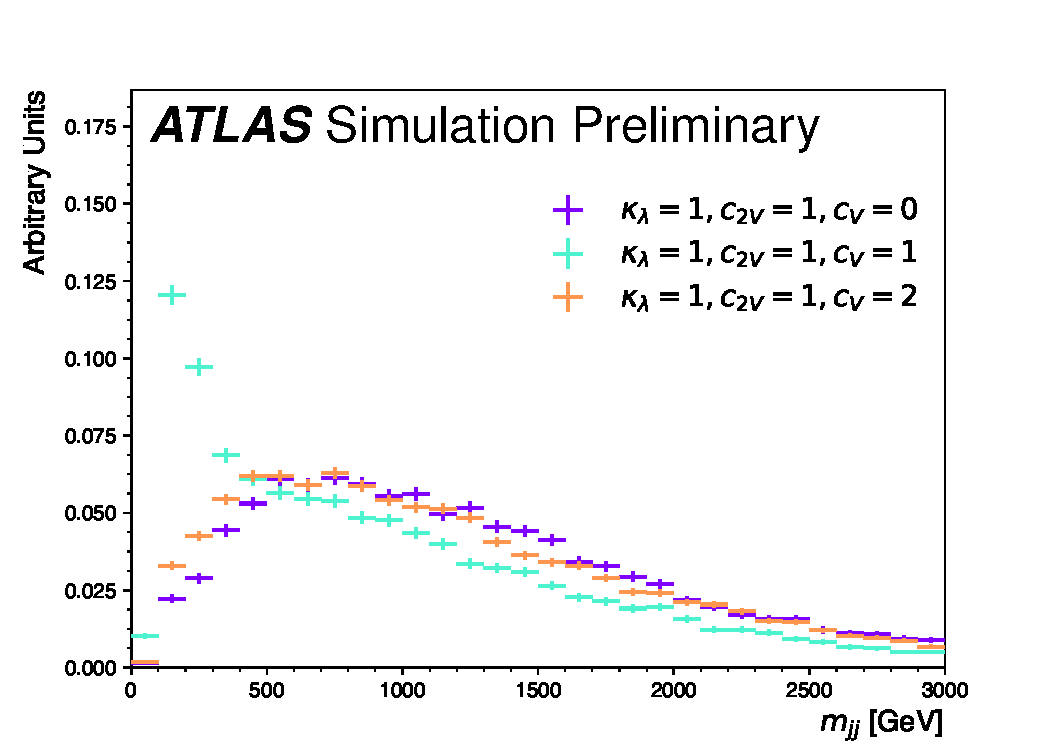
\includegraphics[width=0.33\textwidth]{chapters/chapter6_vbf/images/mc_samples/m_jj_cv.pdf}
    }
    \subfloat{
      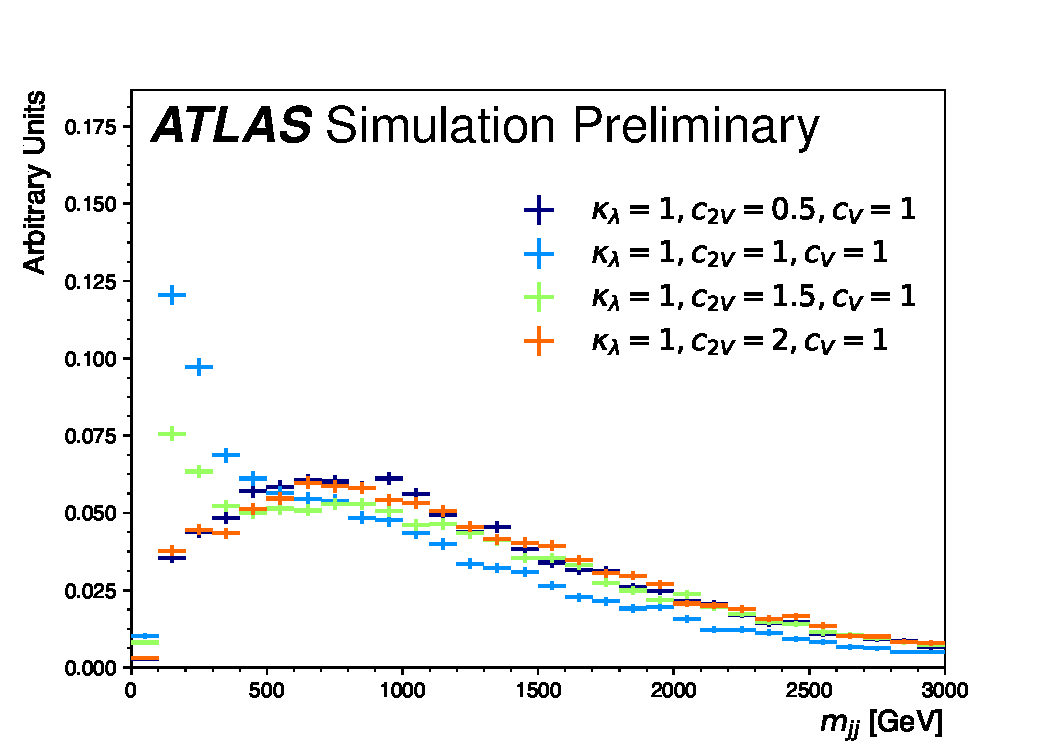
\includegraphics[width= 0.33\textwidth]{chapters/chapter6_vbf/images/mc_samples/m_jj_cvv.pdf}
    }
    \subfloat{
      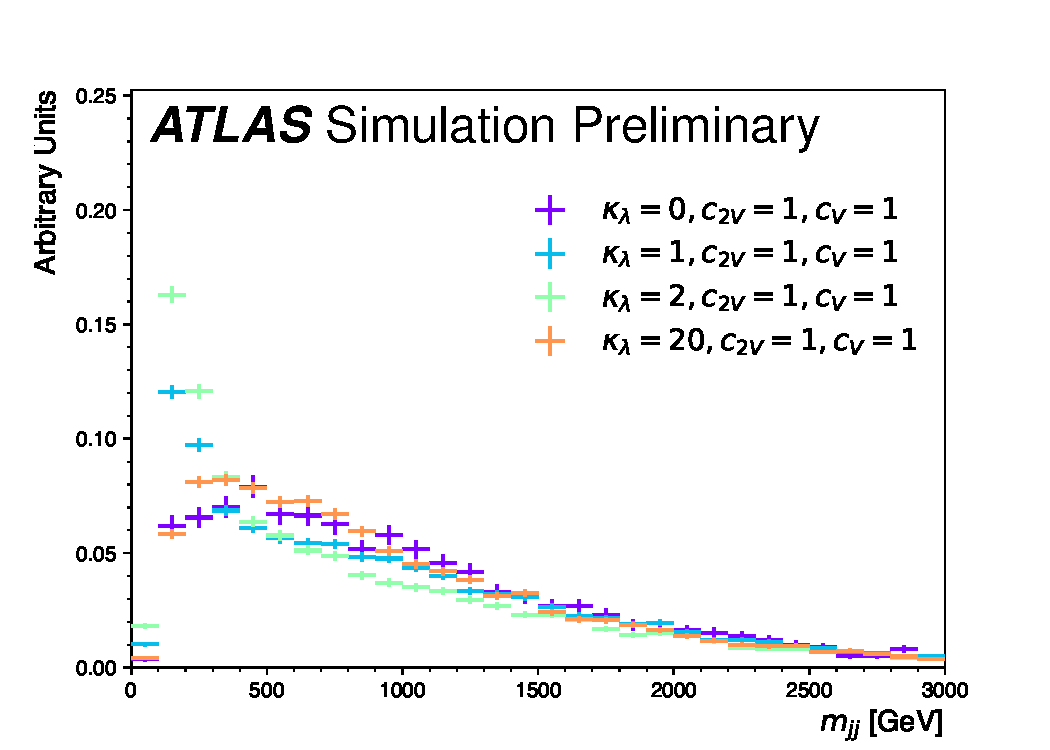
\includegraphics[width= 0.33\textwidth]{chapters/chapter6_vbf/images/mc_samples/m_jj_klambda.pdf}

    }       

    \subfloat{
        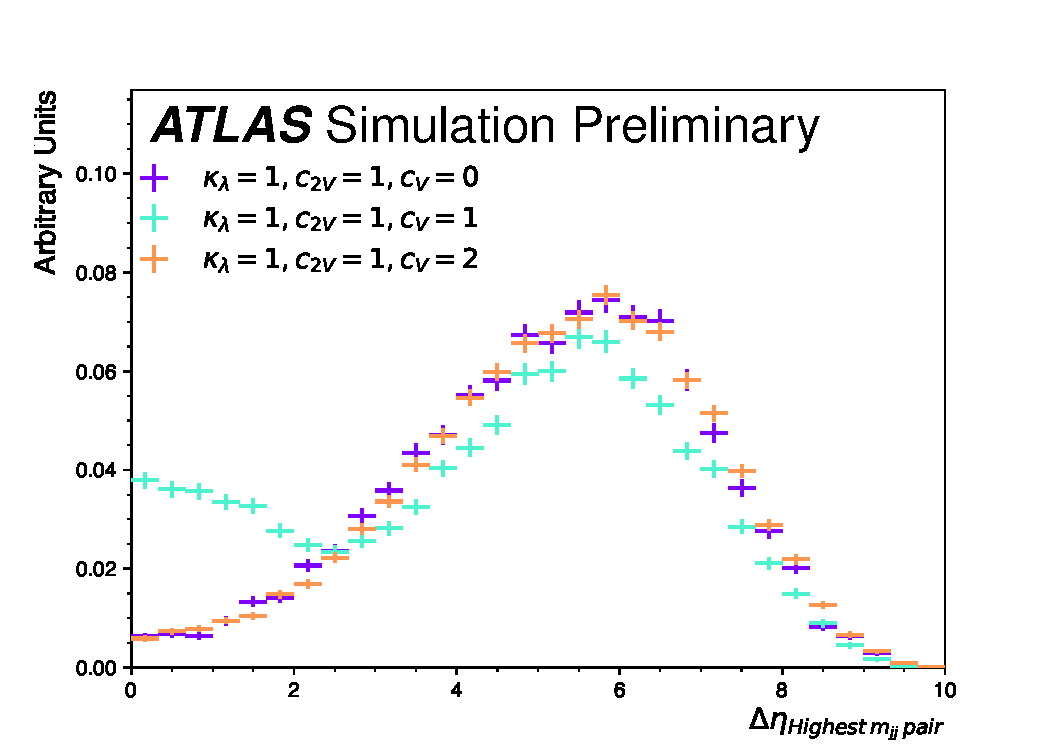
\includegraphics[width=0.33\textwidth]{chapters/chapter6_vbf/images/mc_samples/jj_deta_cv.pdf}
      }
      \subfloat{
        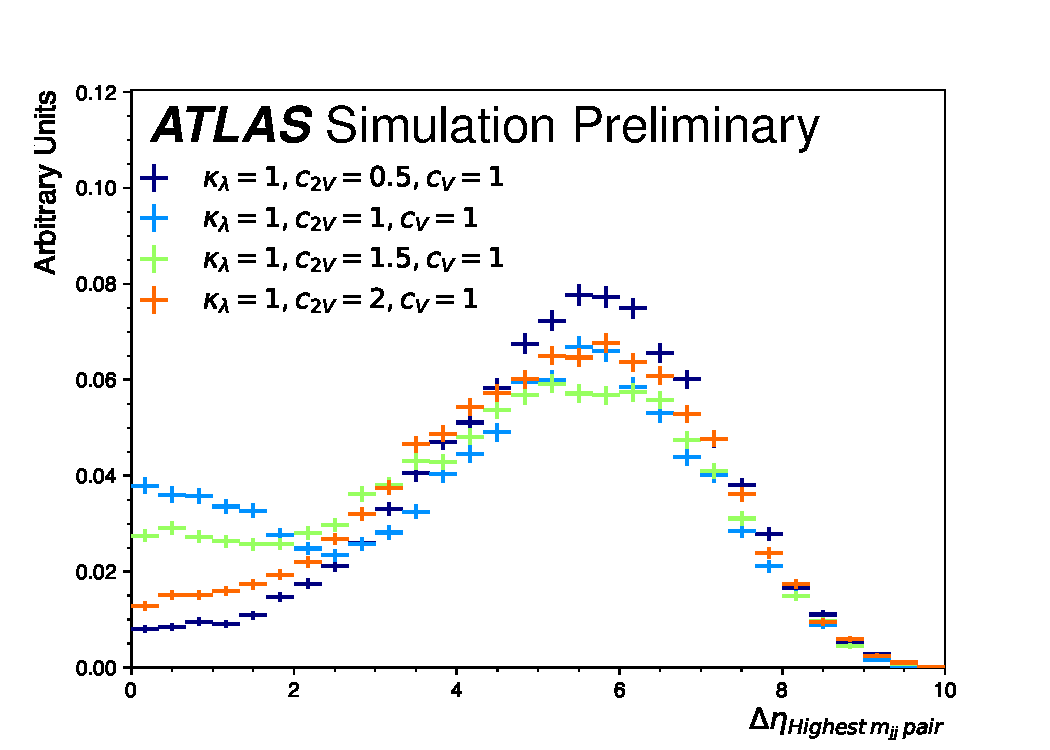
\includegraphics[width= 0.33\textwidth]{chapters/chapter6_vbf/images/mc_samples/jj_deta_cvv.pdf}
      }
      \subfloat{
        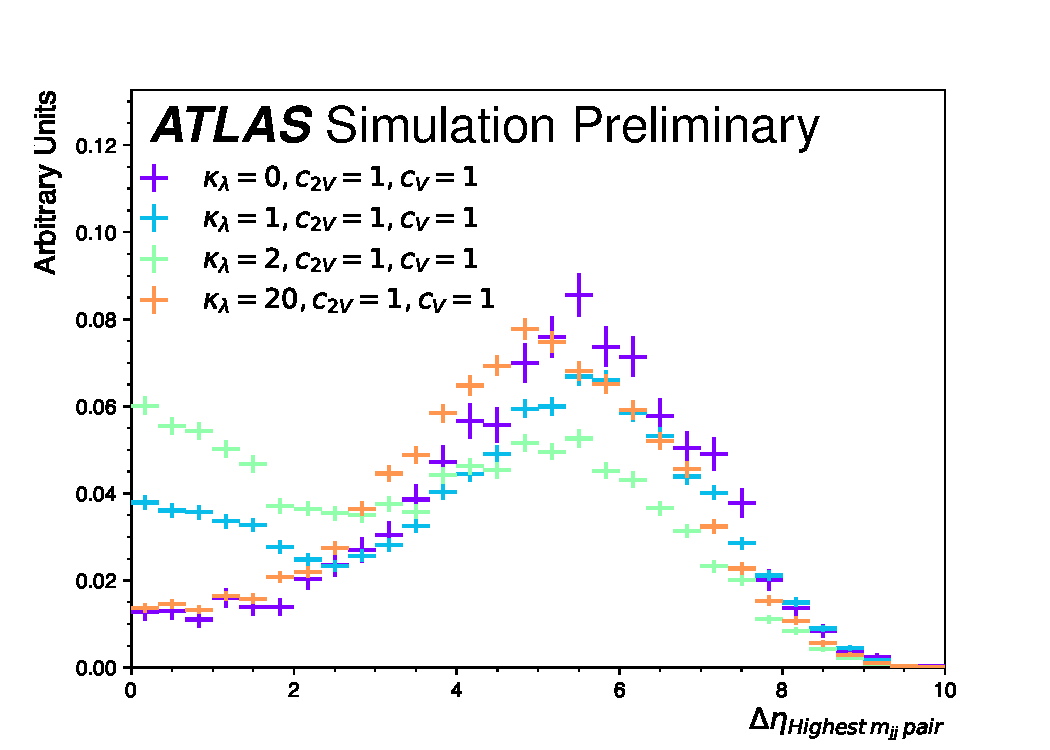
\includegraphics[width= 0.33\textwidth]{chapters/chapter6_vbf/images/mc_samples/jj_deta_klambda.pdf}
    }    

    \caption{Validation plots at parton level for the VBF $HH$ signal sample. The highest $m_{jj}$ pair is selected as a proxy for the VBF jets. The top row shows the invariant mass distribution of this system, the bottom depicts the $\Delta \eta$ between these jets. Left to right, these plots vary the $c_V$, $c_{2V}$, and $\kappa_\lambda$ strength. The peak at low $m_{jj}$ values and shoulder at low $\Delta \eta$ is a product of the $VHH$ hadronic and Higgsstrahlung contributions in the samples.}
    \label{fig:vbf-mc-validation}
\end{figure}

\section{Event Selection} \label{ssec:vbf-event-selection}

To improve the event selection presented in Section \ref{sec:yybb-event-selection} the following method is applied:

First, the following preselection cuts are applied:

\begin{itemize}
	\item $N_{\text{cen jets}} < 6$, to help reject ttH production (hadronic top decays)
	\item $N_{\text{lep}} = 0$, to help reject ttH production (leptonic top decays)
	\item $N_{\text{85 \% b-tags}} >= 2$ 
	\item $N_{\text{70 \% b-tags}} < 3$, to maintain orthogonality with the $HH \rightarrow \bb\bb$ analysis
\end{itemize}

\subsection{BDT for ggF Production}
A \gls{BDT} has been trained in order to maximize signal efficiency for ggF HH production. Following preselection, events are segmented into two regions, a high mass region with $M_X^{*} > 350 \text{GeV}$ targeting the standard model signal, and a low mass region with $M_X^{*} < 350 \text{GeV}$ targeting BSM signals. 

In each region, a separate BDT is trained using a benchmark HH signal against a combination of \yy, $ttH$, $ggH$, and $ZH$ backgrounds. In the high mass region, the standard model HH sample is used as signal, while in the low mass region, the $\klambda = 6$ sample is used as signal.

The following inputs are used:

\begin{itemize}
	\item{The $p_{T}/m_{\yy}$, $\eta$, $\phi$ of the two photons} 
	\item{The $p_{T}$, $\eta$, $\phi$, and pseudo-continuous b-tagging score of the first two jets}
	\item{The MET and the $\phi$ angle of the MET}
	\item{The $p_{T}$, $\eta$, $\phi$, and mass of the $H\rightarrow \bb$ candidate}
	\item{The $H_{T}$ (scalar $p_{T}$ sum of all jets)}
\end{itemize}

Where,

\begin{itemize}
	\item{The $p_{T}$ of the two photons are scaled by $m_{\yy}$ to prevent the BDT from learning the $m_{\yy}$ variable. There is no equivalent scaling done for the two jets, since nominally we only fit to $m_{\yy}$, not $m_{\bb}$.}
	\item{Jets are ordered by pseudo-continuous b-tagging score, and then by $p_{T}$ in case of a tie. The $H \rightarrow \bb$ candidate is then formed by the two highest ranked jets by simply summing their four-vectors.}
	\item{All vectors are rotated by the same $\phi$ angle so that the $\phi$ of the leading photon is equal to zero. This effectively removes one degree of freedom for the BDT to learn.}
\end{itemize}

After training, two categories are created in each mass region by creating cuts on the BDT output. The category boundaries are optimized to give the best Asimov number counting significance \cite{asimov}, given by

\begin{equation}\label{eqn:asimov-significance}
    Z = \sqrt{2[(s+b)\log{(1 + s/b)} -s]}.
\end{equation}


\subsection{BDT for VBF Production}
Atop the ggF \gls{BDT} selection, a dedicated VBF-enriched analysis category is built. Events which have already passed the ggF BDT based selection and have at least 4 jets are considered the VBF category. The 4 jet requirement is imposed in order to reconstruct VBF-based variables, since 2 jets are needed for the \Hbb decay, and another 2 are needed for the VBF jets. The VBF jets are then selected as the highest $m_{jj}$ pairing, excluding $H\rightarrow b\bar{b}$ candidate jets.

These events are then evaluated by a multiclass BDT, which has independent classes for VBF HH, ggF HH, $\gamma \gamma$-continuum, and $ttH$. Ultimately, an event selected for the VBF category if it passes the BDT score threshold for VBF HH, and fails the score threshold for the other three classes. A flowchart of this logic is shown in Figure \ref{fig:vbf-logic}.

\begin{figure}[htbp]
    \centering
	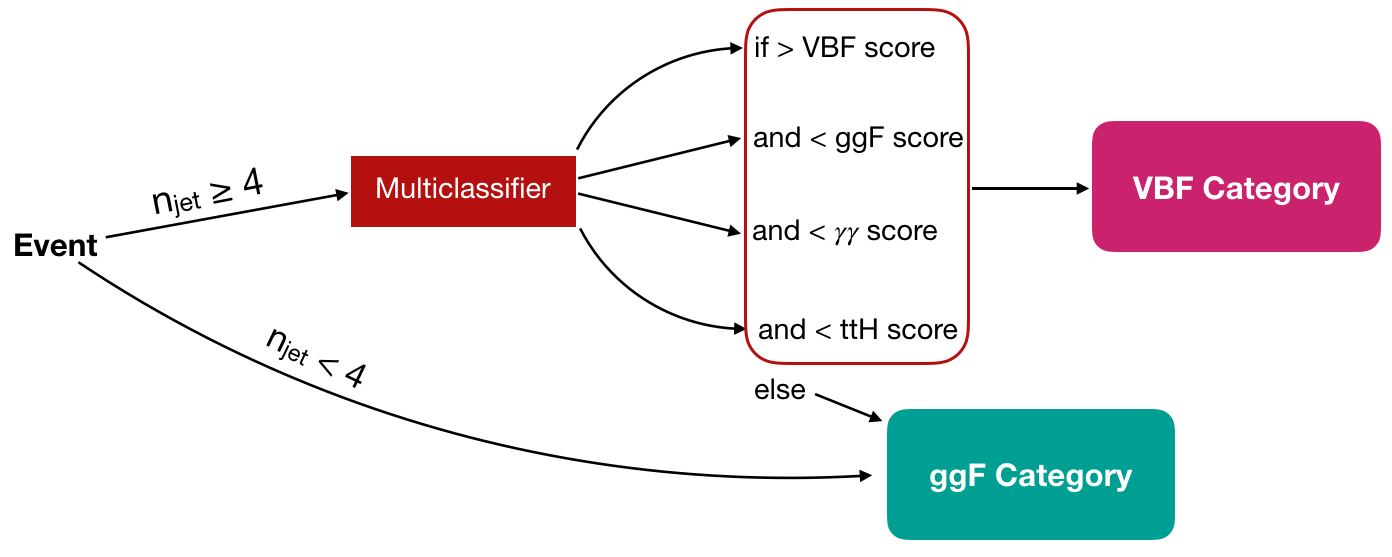
\includegraphics[width=0.9\textwidth]{chapters/chapter6_vbf/images/vbf_logic.png}
    \caption{Logic flow for an event to be selected into the VBF-enriched signal region. The starting set of candidates (denoted ``event'') requires passing preselection and at least one of the ggF-based signal categories. If an event is assigned to the ggF categories, it is separated into 4 categories.}
    \label{fig:vbf-logic}
\end{figure}

\subsubsection{Input Selection}
A set of 26 variables were considered for this BDT, listed in Appendix \ref{app:vbf-variables}. Broadly, they describe the kinematics of various physics objects in the event, as well as event shape variables \cite{STDM-2011-33} and variables to reconstruct the W-mass, which aim to suppress the ttH background.

For dimensionality reduction, a pruning procedure was performed.
\begin{enumerate}
  \item To remove redundant variables, those with a pearson correlation value above 0.85 were removed. This brought the list from 26 to 19, pruning several event shape variables.
  \item After pruning those variables and retraining, low-impact variables were removed. The pearson correlation for each variable to the 4 class \gls{BDT} probability distributions were calculated. Those 4 correlation values were summed, and variables with a sum less than 1.0 were pruned. This brought the set from 19 to 10 input variables.
\end{enumerate}

After this pruning procedure, the 10 final inputs were: 

\textbf{VBF-targeted:} $\Delta \eta_{jj}$, $m_{jj}$

\textbf{$\gamma \gamma$-suppressing:} \myybb, $\Delta R_{\gamma\gamma}$, $\Delta R_{\bb}$, the best b-tagging WP for the $H\rightarrow \bb$ jets

\textbf{$ttH$-suppressing:} Transverse Sphericity ($S_{\perp}$), Planar Flow ($Pf$), $\pt^\text{balance}$

Where $S_{\perp}$ is given in Reference \cite{STDM-2011-33}, Planar Flow is given in Reference \cite{planar-flow}, and $\pt^\text{balance}$ is given by:

\begin{equation} \label{eqn:pt-balance}
    \pt^\text{balance} = \frac
    {| \vec{p}_T^{\ell_1} + \vec{p}_T^{\ell_2} + \vec{p}_T^{j_1} +  \vec{p}_T^{j_2}|}
    {|\vec{p}_T^{\ell_1}| + |\vec{p}_T^{\ell_2}| + |\vec{p}_T^{j_1}| +  |\vec{p}_T^{j_2}|}.
\end{equation}


Distributions for each these variables after applying a 4-jet requirement can be found in Appendix \ref{app:vbf-variables}. 

\subsubsection{Model Optimization}

This subsection outlines two optimizations performed on the \gls{BDT}. First, the selection of model hyperparameters, and second, the selection of cuts on the \gls{BDT} score to define the \gls{VBF} signal category. For these optimizations, an orthogonal sample of events must be selected to ensure the model is generalizable. A subset of 50\% of the data is used for training, 25\% for testing, and 25\% for model selection\footnote{This split is done using the ATLAS global event number. A modulo 4 operation is performed on the event number, if the result is 0 or 1, it is used in the training sample. If the result is 2, it is used in the testing sample. If the result is 3, it is used in the model selection sample.}.

\noindent\textbf{Hyperparameter Optimization}\\
\indent The maximum \gls{BDT} depth is selected at the point in which the accuracy on the testing set maximizes, a depth of 14. After that point, the accuracy on the training set flattens, while it continues to increase on the testing set, leading to overtraining. The same procedure is performed for the number of trees, however this parameter flattens for both training and testing, so a safe choice of 200 trees is used. The accuracy as a function of these parameters is shown in Figure \ref{fig:hp-opt}.

\begin{figure}[!h]
  \centering
  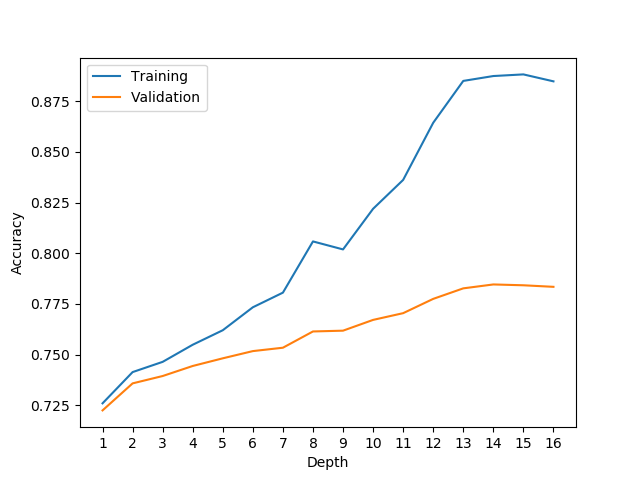
\includegraphics[width=0.48\textwidth]{chapters/chapter6_vbf/images/hp_opt/multiclass_optimized_depth.png}
  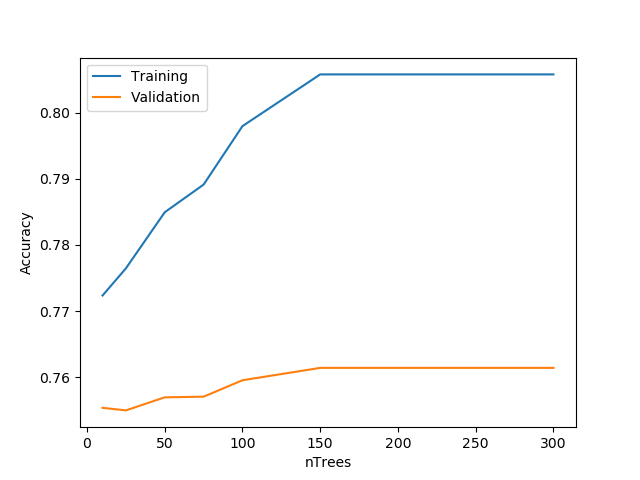
\includegraphics[width=0.48\textwidth]{chapters/chapter6_vbf/images/hp_opt/multiclass_optimized_trees.png}
  \caption[The \gls{BDT} accuracy as a function of hyperparameter values]{The \gls{BDT} accuracy as a function of hyperparameter values. The left is the maximum tree depth, which is chosen to be 14. The right shows the number of trees, which is chosen to be 200.}
  \label{fig:hp-opt}
\end{figure}

\noindent\textbf{BDT Score Cuts}\\
\indent Evaluating an event on this multiclass \gls{BDT} outputs 4 probabilities, one for each class. These are denoted $p_{\text{class}}$ for each target class, e.g. $p_{\text{VBF}}$ for the class targeting VBF HH production. In order to set the thresholds for each of these probabilities, an optimization procedure is performed. A 4-dimensional scan over the 4 probability scores is performed, in steps of 0.03. At each step, the Asimov significance, given in Equation \ref{eqn:asimov-significance}, is calculated for each category and summed in quadrature. In this equation, the signal $s$, is the sum of both ggF and VBF HH contributions in a category. The background, $b$, is the sum of the following considered backgrounds:
\begin{itemize}
  \item \yy-continuum processes
  \item \glsfirst{NTNI} data. This is data that fails either photon identification, isolation, or both. It is proportionally scaled to the sum of the $\gamma j$, $j \gamma$, and $jj$ events derived by the 2x2D method, described in section \ref{ssec:background-composition}.
  \item Top-quark pair production associated with 2 photons, $t\bar{t}\yy$
  \item The leading mono-Higgs backgrounds, $ttH$, $ZH$, and $ggH$.
\end{itemize}

Through this optimization procedure, the thresholds shown in Table \ref{tab:multiclass-thresholds} are found. The output probability distributions for each class on each sample is shown in Figure \ref{fig:bdt-scores}, with the optimized thresholds overlaid.

\begin{table}[!htb]
  \centering
  \caption[The optimized thresholds for each \gls{BDT} score used to define the VBF-enriched category]{The optimized thresholds for each \gls{BDT} score used to define the VBF-enriched category. The cut threshold of 0.00 on the VBF HH class means that this class is not cut on.}
  \begin{tabular}{c|c|c}
    \hline
    Class & Target & Selection Logic  \\
    \hline
    0 & VBF HH & $p_{\text{VBF}} > 0.00 $ \\
    1 & ggF HH & $p_{\text{ggF}} < 0.72 $ \\
    2 & $\gamma\gamma$-Continuum &  $p_{\gamma\gamma} < 0.06$ \\
    3 & $ttH$ &  $p_{ttH} < 0.81$ \\
    \hline
  \end{tabular}
  \label{tab:multiclass-thresholds}
\end{table}

\begin{figure}[!h]
  \centering
  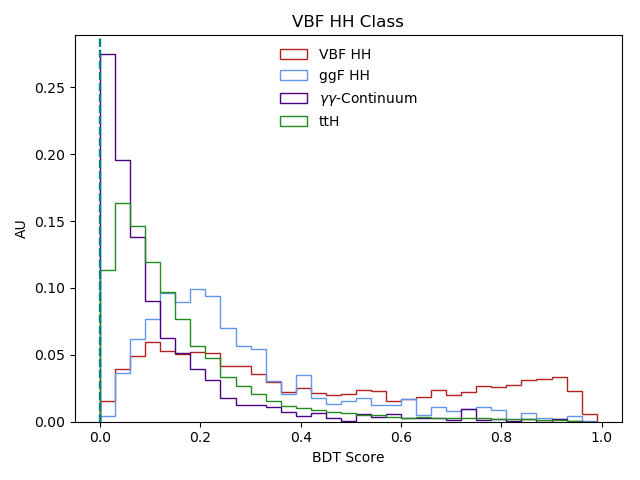
\includegraphics[width=0.48\textwidth]{chapters/chapter6_vbf/images/bdt_scores/vbf_scores.png}
  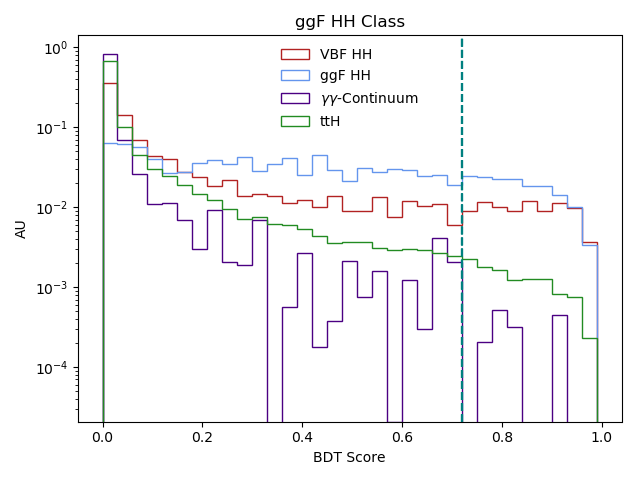
\includegraphics[width=0.48\textwidth]{chapters/chapter6_vbf/images/bdt_scores/log_ggf_scores.png}
  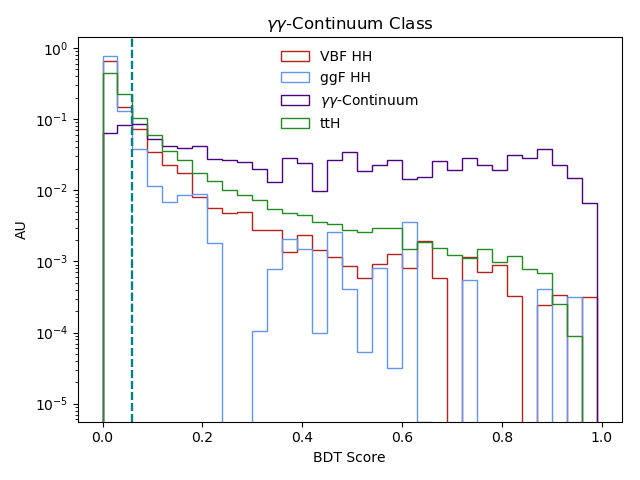
\includegraphics[width=0.48\textwidth]{chapters/chapter6_vbf/images/bdt_scores/log_yy_scores.png}
  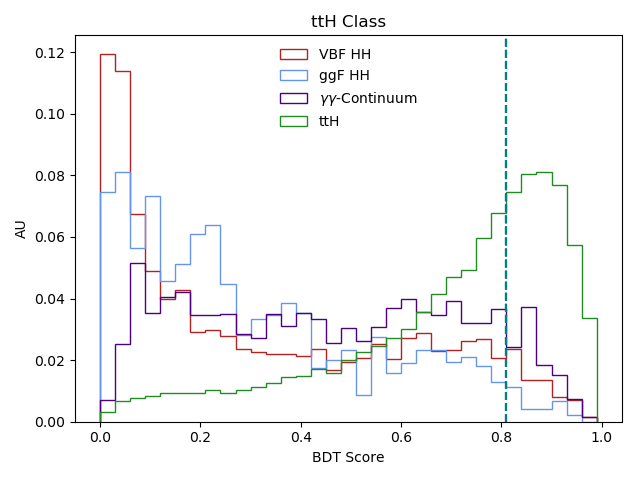
\includegraphics[width=0.48\textwidth]{chapters/chapter6_vbf/images/bdt_scores/tth_scores.png}
  \caption[The \gls{BDT} score distribution for each class, evaluated on the VBF HH, ggF HH, \yy-continuum, and $ttH$ samples]{The \gls{BDT} score distribution for each class, evaluated on the testing VBF HH, ggF HH, \yy-continuum, and $ttH$ samples. The ggF HH and \yy-continuum distributions are shown on a log scale. A vertical line showing the cut threshold is shown on each distribution.}
  \label{fig:bdt-scores}
\end{figure}

The contribution of each signal and background process to each category is shown in Figure \ref{fig:category-yields}.

\begin{figure}[p!]
  \centering
  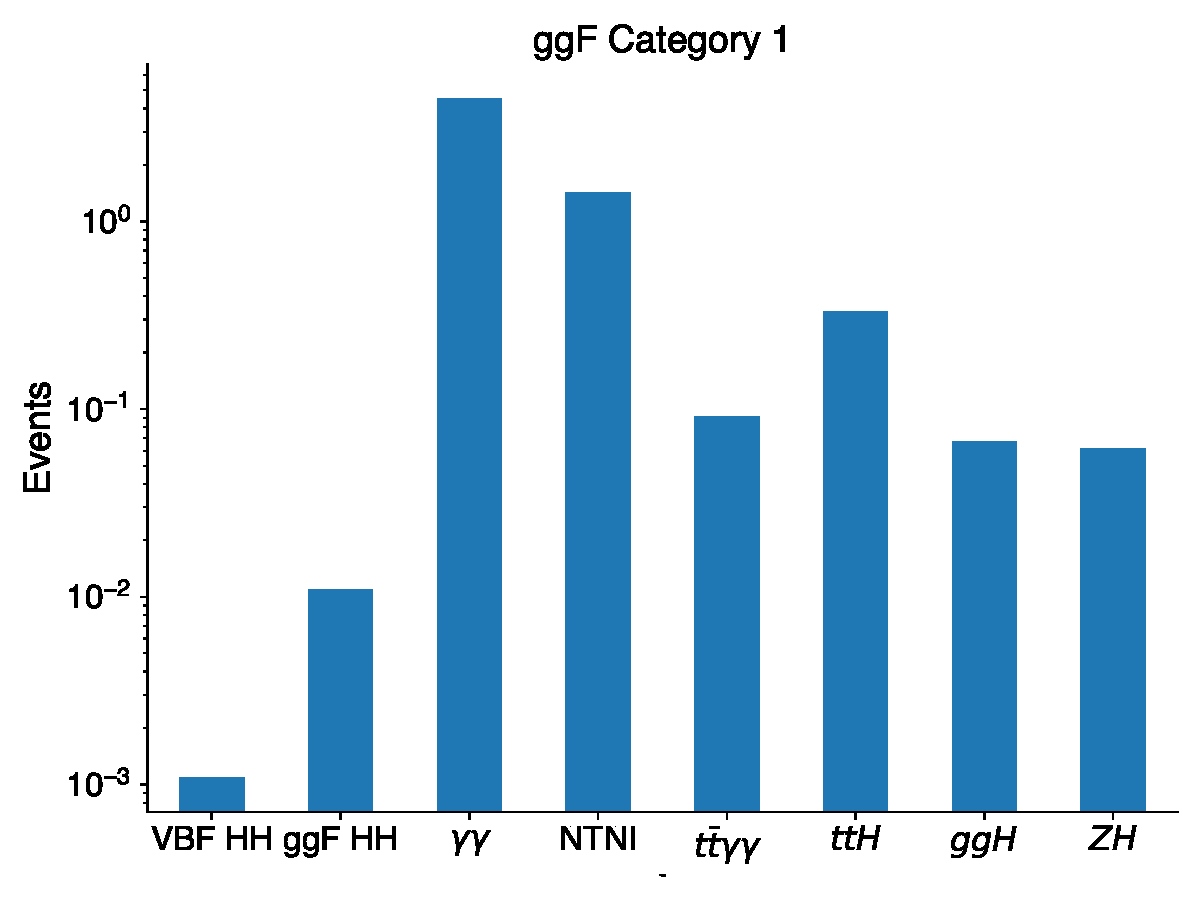
\includegraphics[width=0.48\textwidth]{chapters/chapter6_vbf/images/category_breakdown/ggfcat1.pdf}
  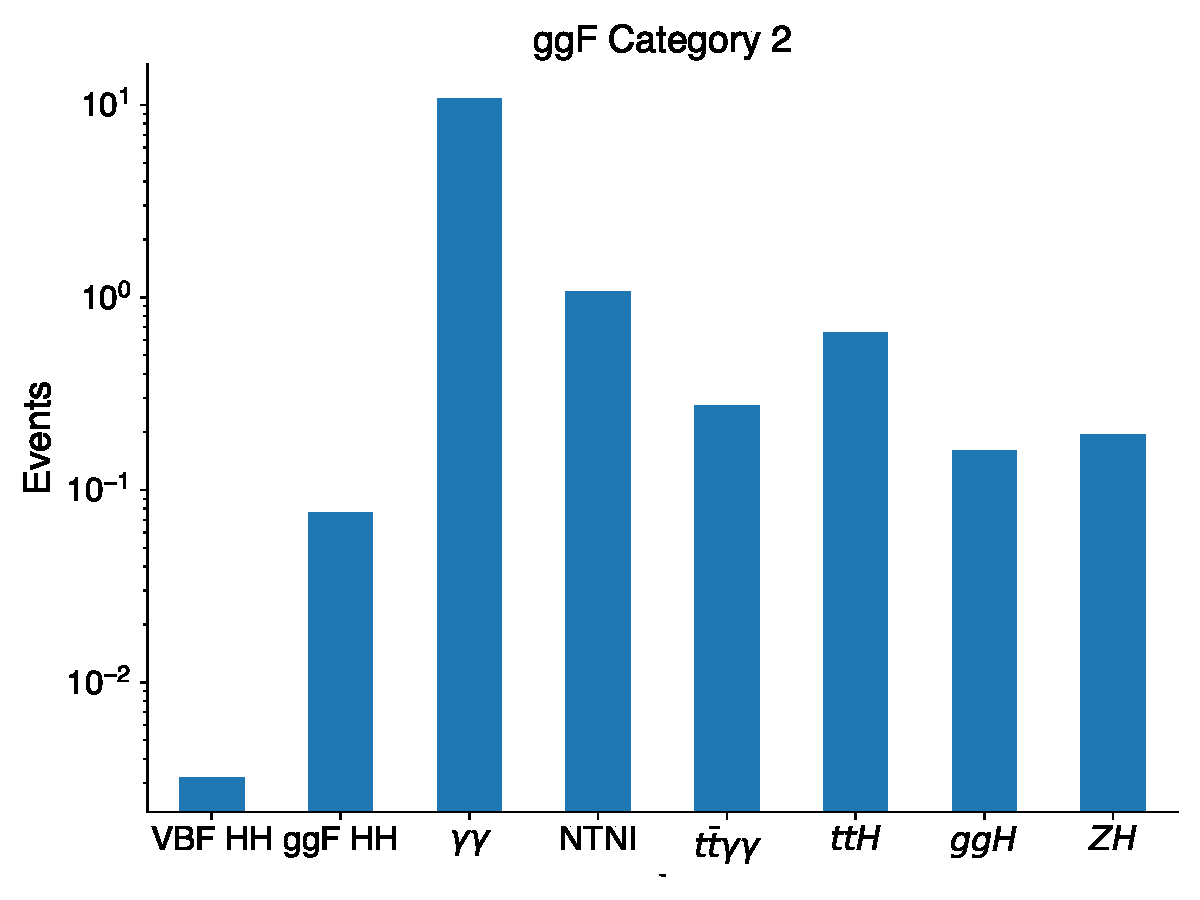
\includegraphics[width=0.48\textwidth]{chapters/chapter6_vbf/images/category_breakdown/ggfcat2.pdf}
  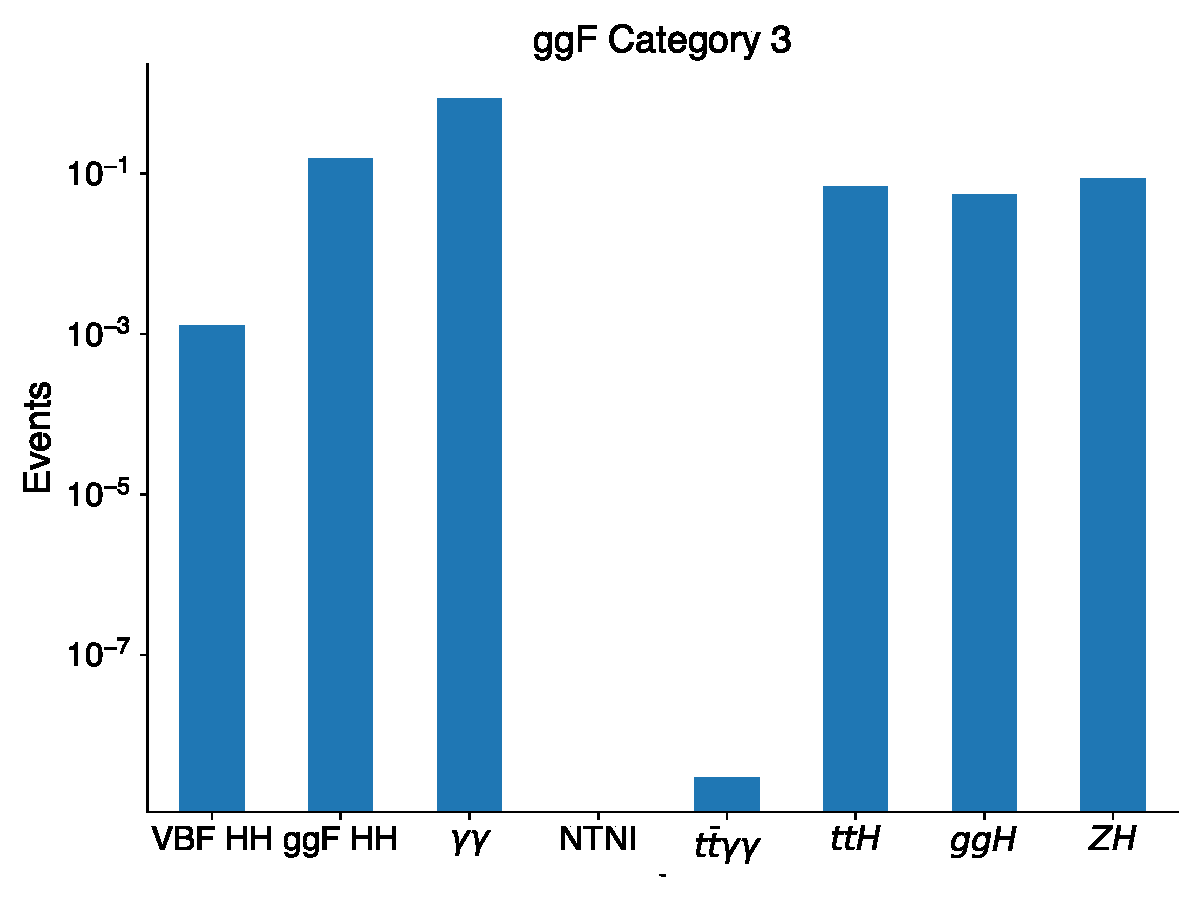
\includegraphics[width=0.48\textwidth]{chapters/chapter6_vbf/images/category_breakdown/ggfcat3.pdf}
  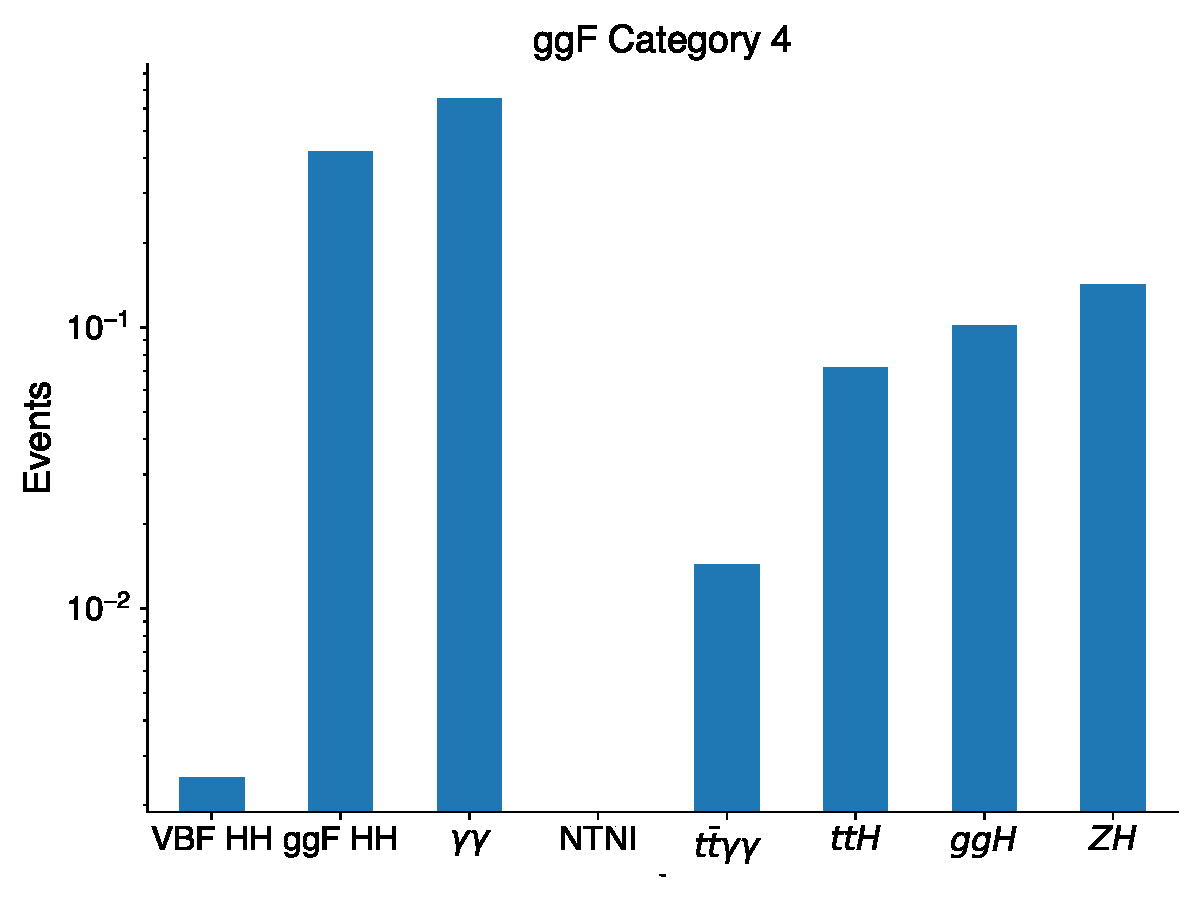
\includegraphics[width=0.48\textwidth]{chapters/chapter6_vbf/images/category_breakdown/ggfcat4.pdf}
  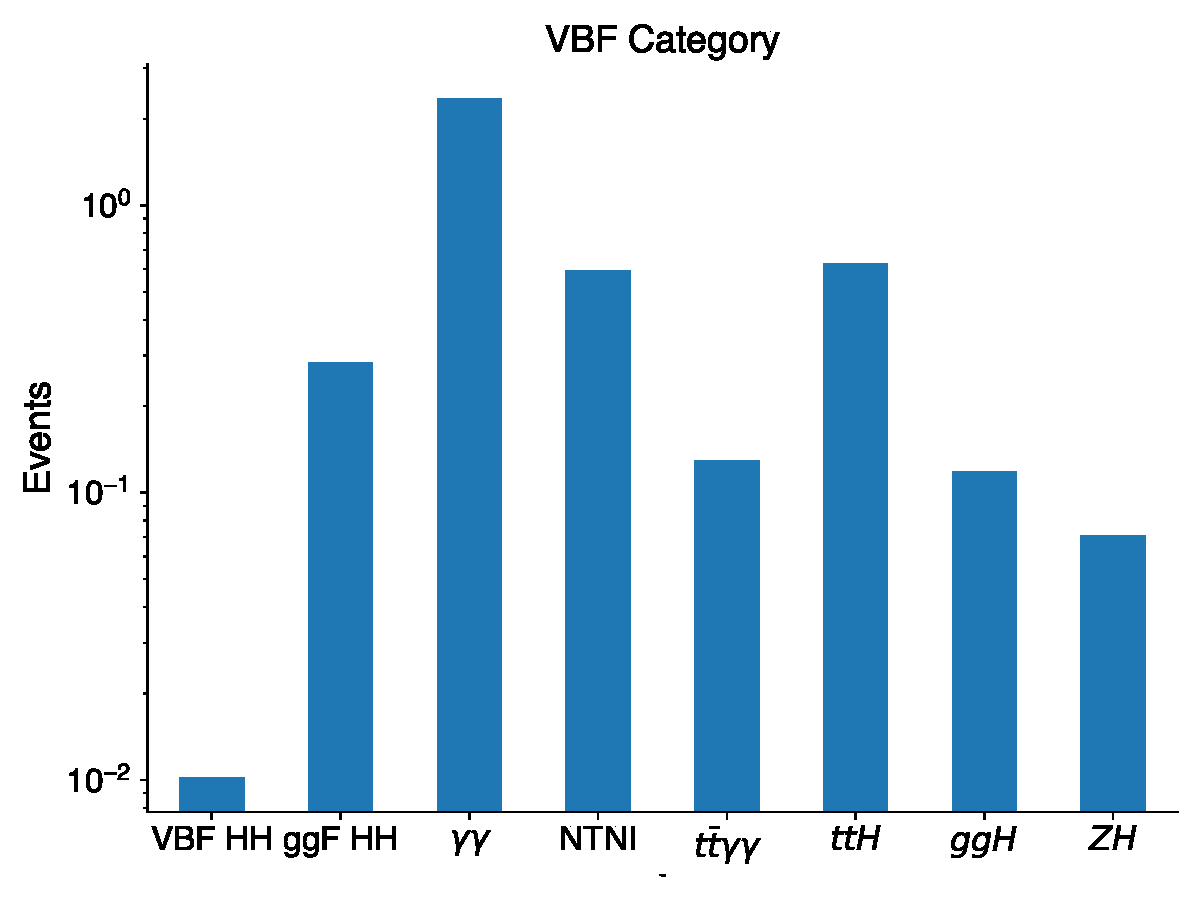
\includegraphics[width=0.48\textwidth]{chapters/chapter6_vbf/images/category_breakdown/vbfcat.pdf}
  \caption[The contribution of signal and leading background samples to each analysis category after adding the optimized VBF-enriched category]{The contribution of signal and leading background samples to each analysis category after adding the optimized VBF-enriched category. VBF and ggF HH are the two considered signal production modes. $\gamma \gamma$ is the diphoton continuum background, $t\bar{t}\gamma\gamma$ is top-quark pair production associated with 2 photons, NTNI is not-tight not-isolated data (scaled using a template fit).  The three dominant mono-Higgs backgrounds, ttH, ggH, and $ZH$ are shown.}
  \label{fig:category-yields}
\end{figure}

The categorization for each signal process as well as the dominant \yy-continuum background is shown in Figure \ref{fig:process-categorization}. The categorization for the mono-Higgs, \gls{NTNI}, and $tt\yy$ samples are shown in Appendix \ref{app:vbf-yield}.

\begin{figure}
  \centering
  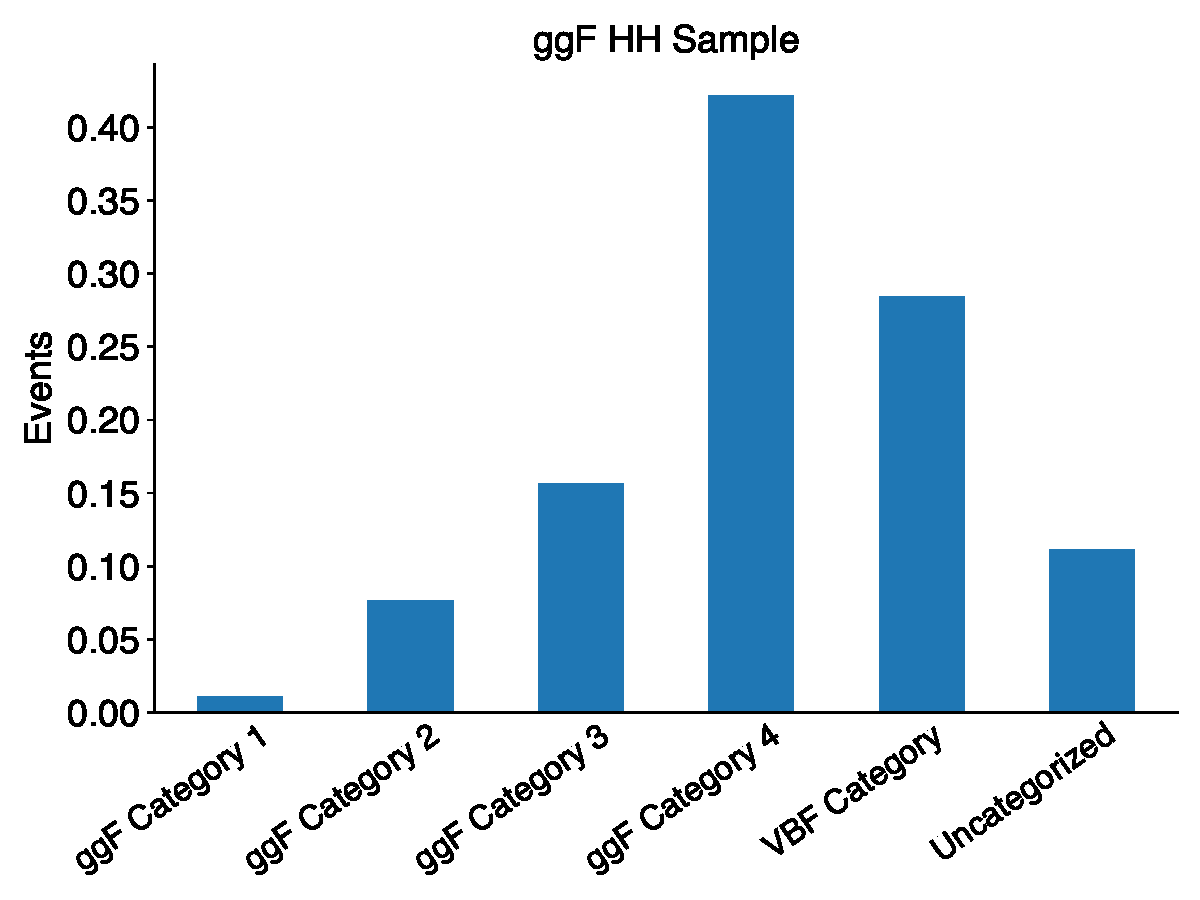
\includegraphics[width=0.48\textwidth]{chapters/chapter6_vbf/images/category_breakdown/ggf_sample.pdf}
  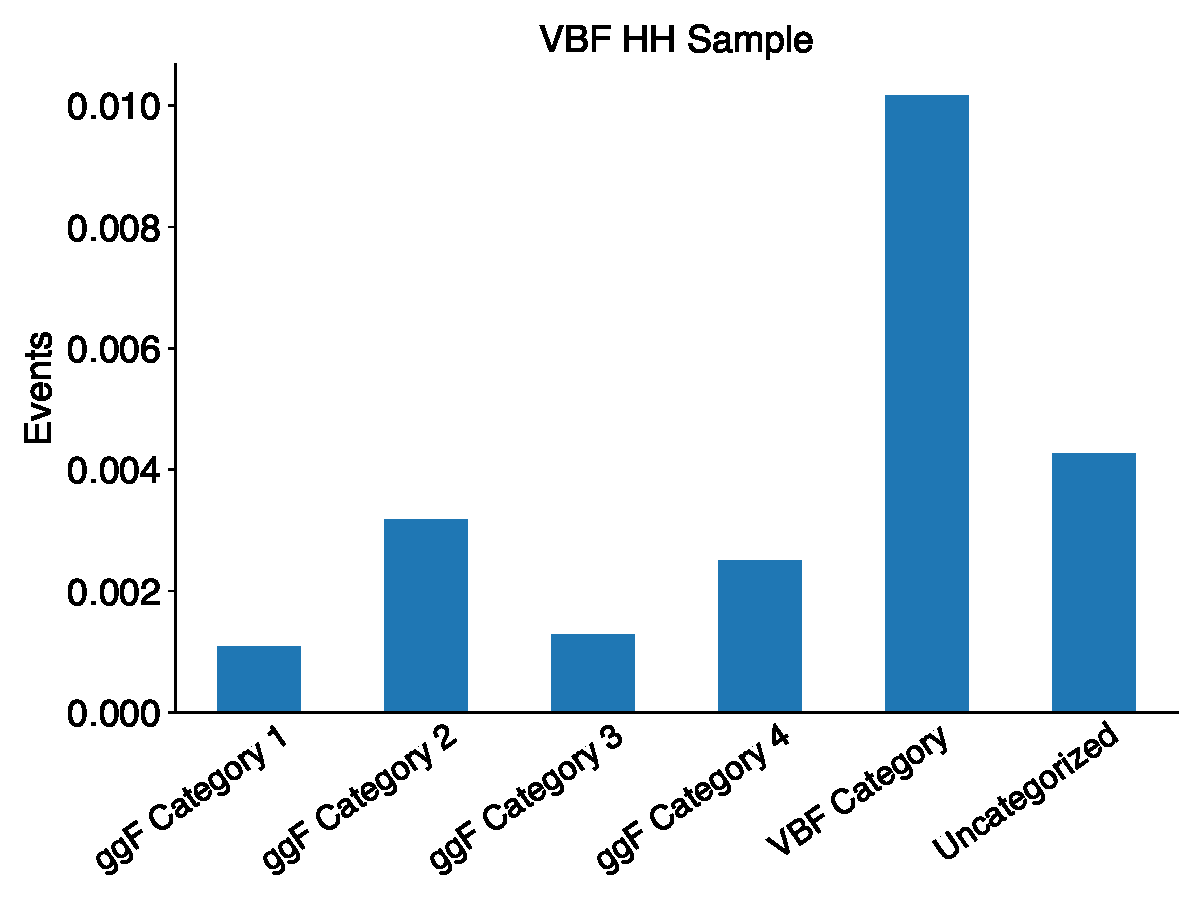
\includegraphics[width=0.48\textwidth]{chapters/chapter6_vbf/images/category_breakdown/vbf_sample.pdf}
  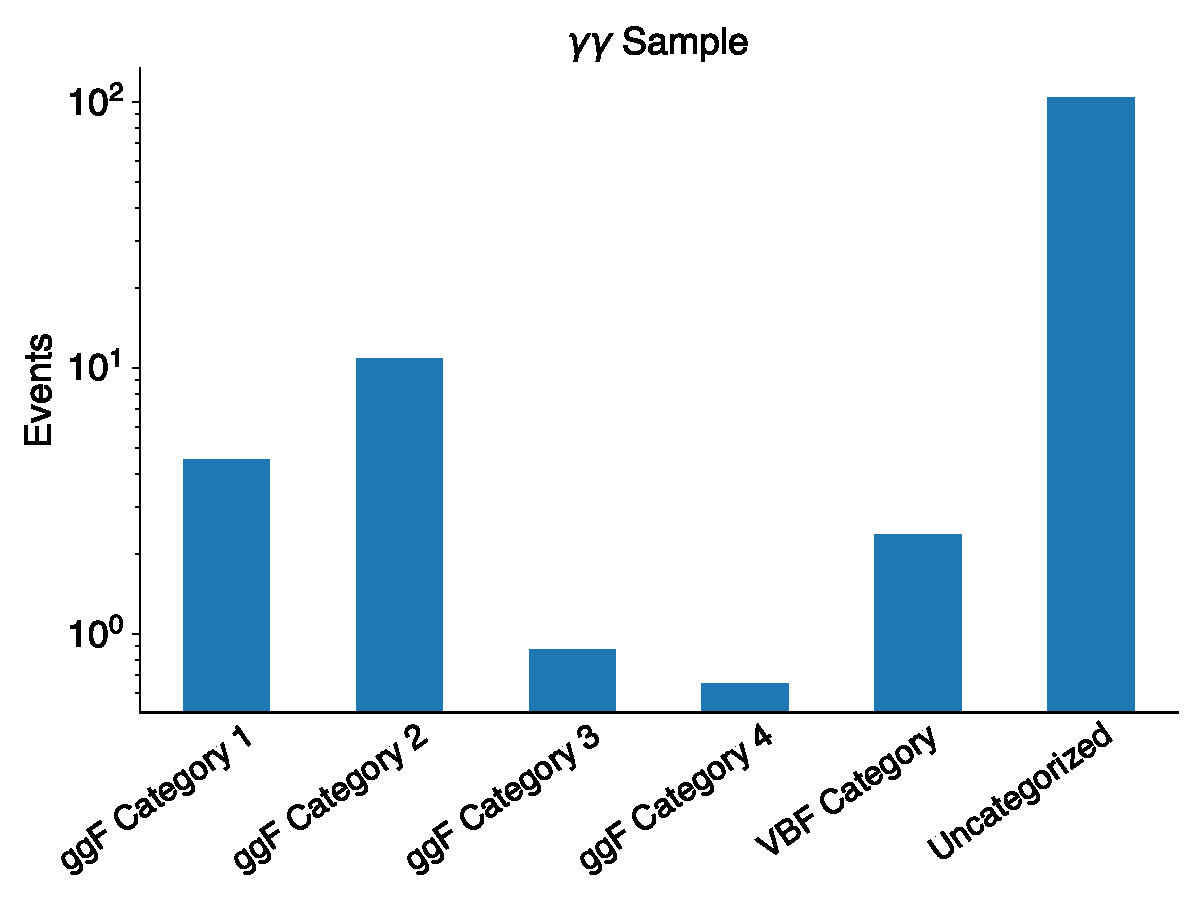
\includegraphics[width=0.48\textwidth]{chapters/chapter6_vbf/images/category_breakdown/yy_sample.pdf}
  \caption[The categorization of the VBF HH, ggF HH, and \yy-continuum samples]{The categorization of the VBF HH, ggF HH, and \yy-continuum samples. The ``Uncategorized'' bin are events which do not fall into any of the analysis categories. The \yy-continuum plot is shown with log-scale.
  \label{fig:process-categorization}}
\end{figure}

By Asimov Significance, equation \ref{eqn:asimov-significance}, adding a VBF-enriched category provides a XXX percent improvement over not defining such a category.

